\documentclass[twoside]{book}

% Packages required by doxygen
\usepackage{fixltx2e}
\usepackage{calc}
\usepackage{doxygen}
\usepackage[export]{adjustbox} % also loads graphicx
\usepackage{graphicx}
\usepackage[utf8]{inputenc}
\usepackage{makeidx}
\usepackage{multicol}
\usepackage{multirow}
\PassOptionsToPackage{warn}{textcomp}
\usepackage{textcomp}
\usepackage[nointegrals]{wasysym}
\usepackage[table]{xcolor}

% Font selection
\usepackage[T1]{fontenc}
\usepackage[scaled=.90]{helvet}
\usepackage{courier}
\usepackage{amssymb}
\usepackage{sectsty}
\renewcommand{\familydefault}{\sfdefault}
\allsectionsfont{%
  \fontseries{bc}\selectfont%
  \color{darkgray}%
}
\renewcommand{\DoxyLabelFont}{%
  \fontseries{bc}\selectfont%
  \color{darkgray}%
}
\newcommand{\+}{\discretionary{\mbox{\scriptsize$\hookleftarrow$}}{}{}}

% Page & text layout
\usepackage{geometry}
\geometry{%
  a4paper,%
  top=2.5cm,%
  bottom=2.5cm,%
  left=2.5cm,%
  right=2.5cm%
}
\tolerance=750
\hfuzz=15pt
\hbadness=750
\setlength{\emergencystretch}{15pt}
\setlength{\parindent}{0cm}
\setlength{\parskip}{3ex plus 2ex minus 2ex}
\makeatletter
\renewcommand{\paragraph}{%
  \@startsection{paragraph}{4}{0ex}{-1.0ex}{1.0ex}{%
    \normalfont\normalsize\bfseries\SS@parafont%
  }%
}
\renewcommand{\subparagraph}{%
  \@startsection{subparagraph}{5}{0ex}{-1.0ex}{1.0ex}{%
    \normalfont\normalsize\bfseries\SS@subparafont%
  }%
}
\makeatother

% Headers & footers
\usepackage{fancyhdr}
\pagestyle{fancyplain}
\fancyhead[LE]{\fancyplain{}{\bfseries\thepage}}
\fancyhead[CE]{\fancyplain{}{}}
\fancyhead[RE]{\fancyplain{}{\bfseries\leftmark}}
\fancyhead[LO]{\fancyplain{}{\bfseries\rightmark}}
\fancyhead[CO]{\fancyplain{}{}}
\fancyhead[RO]{\fancyplain{}{\bfseries\thepage}}
\fancyfoot[LE]{\fancyplain{}{}}
\fancyfoot[CE]{\fancyplain{}{}}
\fancyfoot[RE]{\fancyplain{}{\bfseries\scriptsize Generated by Doxygen }}
\fancyfoot[LO]{\fancyplain{}{\bfseries\scriptsize Generated by Doxygen }}
\fancyfoot[CO]{\fancyplain{}{}}
\fancyfoot[RO]{\fancyplain{}{}}
\renewcommand{\footrulewidth}{0.4pt}
\renewcommand{\chaptermark}[1]{%
  \markboth{#1}{}%
}
\renewcommand{\sectionmark}[1]{%
  \markright{\thesection\ #1}%
}

% Indices & bibliography
\usepackage{natbib}
\usepackage[titles]{tocloft}
\setcounter{tocdepth}{3}
\setcounter{secnumdepth}{5}
\makeindex

% Hyperlinks (required, but should be loaded last)
\usepackage{ifpdf}
\ifpdf
  \usepackage[pdftex,pagebackref=true]{hyperref}
\else
  \usepackage[ps2pdf,pagebackref=true]{hyperref}
\fi
\hypersetup{%
  colorlinks=true,%
  linkcolor=blue,%
  citecolor=blue,%
  unicode%
}

% Custom commands
\newcommand{\clearemptydoublepage}{%
  \newpage{\pagestyle{empty}\cleardoublepage}%
}

\usepackage{caption}
\captionsetup{labelsep=space,justification=centering,font={bf},singlelinecheck=off,skip=4pt,position=top}

%===== C O N T E N T S =====

\begin{document}

% Titlepage & ToC
\hypersetup{pageanchor=false,
             bookmarksnumbered=true,
             pdfencoding=unicode
            }
\pagenumbering{roman}
\begin{titlepage}
\vspace*{7cm}
\begin{center}%
{\Large My Project }\\
\vspace*{1cm}
{\large Generated by Doxygen 1.8.11}\\
\end{center}
\end{titlepage}
\clearemptydoublepage
\tableofcontents
\clearemptydoublepage
\pagenumbering{arabic}
\hypersetup{pageanchor=true}

%--- Begin generated contents ---
\chapter{Hierarchical Index}
\section{Class Hierarchy}
This inheritance list is sorted roughly, but not completely, alphabetically\+:\begin{DoxyCompactList}
\item \contentsline{section}{Q\+Widget}{\pageref{classQWidget}}{}
\begin{DoxyCompactList}
\item \contentsline{section}{Login\+Window}{\pageref{classLoginWindow}}{}
\item \contentsline{section}{Pop\+Error}{\pageref{classPopError}}{}
\item \contentsline{section}{Registration\+Window}{\pageref{classRegistrationWindow}}{}
\end{DoxyCompactList}
\end{DoxyCompactList}

\chapter{Class Index}
\section{Class List}
Here are the classes, structs, unions and interfaces with brief descriptions\+:\begin{DoxyCompactList}
\item\contentsline{section}{\hyperlink{classLoginWindow}{Login\+Window} \\*Class which creates the G\+UI for login window }{\pageref{classLoginWindow}}{}
\item\contentsline{section}{\hyperlink{classRegistrationWindow}{Registration\+Window} }{\pageref{classRegistrationWindow}}{}
\end{DoxyCompactList}

\chapter{File Index}
\section{File List}
Here is a list of all documented files with brief descriptions\+:\begin{DoxyCompactList}
\item\contentsline{section}{\hyperlink{LoginWindow_8hpp}{Login\+Window.\+hpp} }{\pageref{LoginWindow_8hpp}}{}
\item\contentsline{section}{{\bfseries Registration\+Window.\+hpp} }{\pageref{RegistrationWindow_8hpp}}{}
\end{DoxyCompactList}

\chapter{Class Documentation}
\hypertarget{classLoginWindow}{}\section{Login\+Window Class Reference}
\label{classLoginWindow}\index{Login\+Window@{Login\+Window}}


\hyperlink{classLoginWindow}{Login\+Window} class which creates the G\+UI for login window.  




{\ttfamily \#include $<$Login\+Window.\+hpp$>$}



Inheritance diagram for Login\+Window\+:
% FIG 0


Collaboration diagram for Login\+Window\+:
% FIG 1
\subsection*{Public Types}
\begin{DoxyCompactItemize}
\item 
typedef std\+::string {\bfseries String}\hypertarget{classLoginWindow_a9d5191a38906ea9c5375c1029cfd9d4d}{}\label{classLoginWindow_a9d5191a38906ea9c5375c1029cfd9d4d}

\end{DoxyCompactItemize}
\subsection*{Public Slots}
\begin{DoxyCompactItemize}
\item 
void {\bfseries open\+Reg\+Win} ()\hypertarget{classLoginWindow_abe06ec97d678045c810e2ac6033ee9c0}{}\label{classLoginWindow_abe06ec97d678045c810e2ac6033ee9c0}

\item 
void {\bfseries check\+Login} (const Q\+String \&)\hypertarget{classLoginWindow_a01edb22f1bf6dfdf3bd0811f6c878330}{}\label{classLoginWindow_a01edb22f1bf6dfdf3bd0811f6c878330}

\item 
void \hyperlink{classLoginWindow_ad5a16b9244af77d36f98a4f48d3d423d}{check\+Password} (const Q\+String \&)
\item 
void {\bfseries send\+Login\+Req} ()\hypertarget{classLoginWindow_ac6dc94a63017e4e500b7ec0cbd4cac33}{}\label{classLoginWindow_ac6dc94a63017e4e500b7ec0cbd4cac33}

\end{DoxyCompactItemize}
\subsection*{Public Member Functions}
\begin{DoxyCompactItemize}
\item 
\hyperlink{classLoginWindow_ad3f4ec97bdb1fd55e3e6f6f25112f9d8}{Login\+Window} (Controller \&)
\begin{DoxyCompactList}\small\item\em \hyperlink{classLoginWindow}{Login\+Window} constructor for class \hyperlink{classLoginWindow}{Login\+Window} which creates G\+UI for login window. \end{DoxyCompactList}\item 
void \hyperlink{classLoginWindow_a1d429ebfb0f2ebb21591b209da5d4ecb}{close\+Reg\+Window} ()
\begin{DoxyCompactList}\small\item\em close\+Reg\+Window closing registration window \end{DoxyCompactList}\end{DoxyCompactItemize}


\subsection{Detailed Description}
\hyperlink{classLoginWindow}{Login\+Window} class which creates the G\+UI for login window. 

\subsection{Constructor \& Destructor Documentation}
\index{Login\+Window@{Login\+Window}!Login\+Window@{Login\+Window}}
\index{Login\+Window@{Login\+Window}!Login\+Window@{Login\+Window}}
\subsubsection[{\texorpdfstring{Login\+Window(\+Controller \&)}{LoginWindow(Controller &)}}]{\setlength{\rightskip}{0pt plus 5cm}Login\+Window\+::\+Login\+Window (
\begin{DoxyParamCaption}
\item[{Controller \&}]{c}
\end{DoxyParamCaption}
)}\hypertarget{classLoginWindow_ad3f4ec97bdb1fd55e3e6f6f25112f9d8}{}\label{classLoginWindow_ad3f4ec97bdb1fd55e3e6f6f25112f9d8}


\hyperlink{classLoginWindow}{Login\+Window} constructor for class \hyperlink{classLoginWindow}{Login\+Window} which creates G\+UI for login window. 


\begin{DoxyParams}{Parameters}
{\em is} & an initialized.... ?? \\
\hline
\end{DoxyParams}


\subsection{Member Function Documentation}
\index{Login\+Window@{Login\+Window}!check\+Password@{check\+Password}}
\index{check\+Password@{check\+Password}!Login\+Window@{Login\+Window}}
\subsubsection[{\texorpdfstring{check\+Password}{checkPassword}}]{\setlength{\rightskip}{0pt plus 5cm}void Login\+Window\+::check\+Password (
\begin{DoxyParamCaption}
\item[{const Q\+String \&}]{qs}
\end{DoxyParamCaption}
)\hspace{0.3cm}{\ttfamily [slot]}}\hypertarget{classLoginWindow_ad5a16b9244af77d36f98a4f48d3d423d}{}\label{classLoginWindow_ad5a16b9244af77d36f98a4f48d3d423d}
???????? \index{Login\+Window@{Login\+Window}!close\+Reg\+Window@{close\+Reg\+Window}}
\index{close\+Reg\+Window@{close\+Reg\+Window}!Login\+Window@{Login\+Window}}
\subsubsection[{\texorpdfstring{close\+Reg\+Window()}{closeRegWindow()}}]{\setlength{\rightskip}{0pt plus 5cm}void Login\+Window\+::close\+Reg\+Window (
\begin{DoxyParamCaption}
{}
\end{DoxyParamCaption}
)}\hypertarget{classLoginWindow_a1d429ebfb0f2ebb21591b209da5d4ecb}{}\label{classLoginWindow_a1d429ebfb0f2ebb21591b209da5d4ecb}


close\+Reg\+Window closing registration window 


\begin{DoxyParams}{Parameters}
{\em no} & parametrs \\
\hline
\end{DoxyParams}
\begin{DoxyReturn}{Returns}
void 
\end{DoxyReturn}


The documentation for this class was generated from the following files\+:\begin{DoxyCompactItemize}
\item 
\hyperlink{LoginWindow_8hpp}{Login\+Window.\+hpp}\item 
Login\+Window.\+cpp\end{DoxyCompactItemize}

\hypertarget{classRegistrationWindow}{}\section{Registration\+Window Class Reference}
\label{classRegistrationWindow}\index{Registration\+Window@{Registration\+Window}}


\hyperlink{classRegistrationWindow}{Registration\+Window} class which creates the G\+UI for login window.  




{\ttfamily \#include $<$Registration\+Window.\+hpp$>$}



Inheritance diagram for Registration\+Window\+:
\nopagebreak
\begin{figure}[H]
\begin{center}
\leavevmode
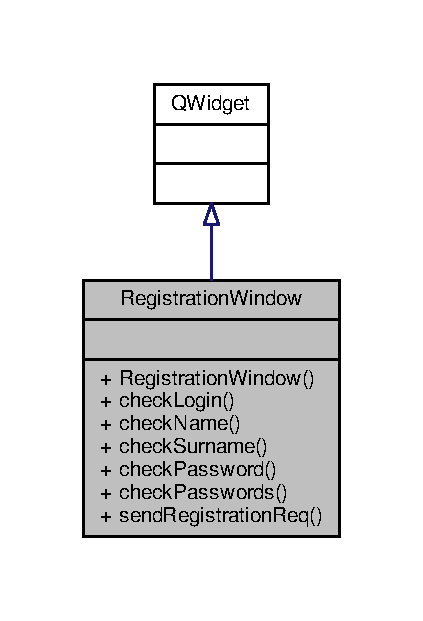
\includegraphics[width=203pt]{classRegistrationWindow__inherit__graph}
\end{center}
\end{figure}


Collaboration diagram for Registration\+Window\+:
\nopagebreak
\begin{figure}[H]
\begin{center}
\leavevmode
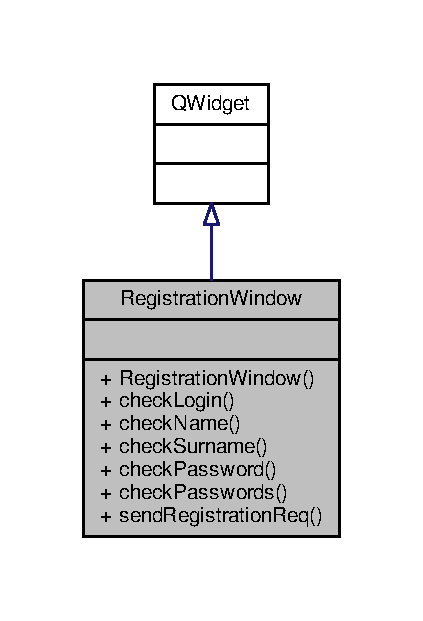
\includegraphics[width=203pt]{classRegistrationWindow__coll__graph}
\end{center}
\end{figure}
\subsection*{Public Types}
\begin{DoxyCompactItemize}
\item 
using \hyperlink{classRegistrationWindow_af737e72502243796bee87789c8b5b9ea}{String} = std\+::string
\end{DoxyCompactItemize}
\subsection*{Public Slots}
\begin{DoxyCompactItemize}
\item 
void \hyperlink{classRegistrationWindow_a054fcf4544f917e106aa6760f720d7b2}{check\+Login} (const Q\+String \&)
\item 
void \hyperlink{classRegistrationWindow_a26d58595ac8df47a0456878a80c45ffc}{check\+Name} (const Q\+String \&)
\item 
void \hyperlink{classRegistrationWindow_a6fc9f673b5e1d2fd15c9e12bfc0174b2}{check\+Surname} (const Q\+String \&)
\item 
void \hyperlink{classRegistrationWindow_a761ec197a38b335aaa5db06287361849}{check\+Password} (const Q\+String \&)
\item 
void \hyperlink{classRegistrationWindow_a6c3761195b00134d3ef4decf91ea76e7}{check\+Passwords} (const Q\+String \&)
\item 
void \hyperlink{classRegistrationWindow_a4344e4dafa6ab47e564c243b20a0c7a4}{send\+Registration\+Req} ()
\end{DoxyCompactItemize}
\subsection*{Public Member Functions}
\begin{DoxyCompactItemize}
\item 
\hyperlink{classRegistrationWindow_ac8876ad29199208fc8b8bd25863c9318}{Registration\+Window} (Controller \&)
\begin{DoxyCompactList}\small\item\em \hyperlink{classRegistrationWindow}{Registration\+Window} constructor for class \hyperlink{classRegistrationWindow}{Registration\+Window} which creates G\+UI for registration window. \end{DoxyCompactList}\end{DoxyCompactItemize}


\subsection{Detailed Description}
\hyperlink{classRegistrationWindow}{Registration\+Window} class which creates the G\+UI for login window. 

\subsection{Member Typedef Documentation}
\index{Registration\+Window@{Registration\+Window}!String@{String}}
\index{String@{String}!Registration\+Window@{Registration\+Window}}
\subsubsection[{\texorpdfstring{String}{String}}]{\setlength{\rightskip}{0pt plus 5cm}using {\bf Registration\+Window\+::\+String} =  std\+::string}\hypertarget{classRegistrationWindow_af737e72502243796bee87789c8b5b9ea}{}\label{classRegistrationWindow_af737e72502243796bee87789c8b5b9ea}


\subsection{Constructor \& Destructor Documentation}
\index{Registration\+Window@{Registration\+Window}!Registration\+Window@{Registration\+Window}}
\index{Registration\+Window@{Registration\+Window}!Registration\+Window@{Registration\+Window}}
\subsubsection[{\texorpdfstring{Registration\+Window(\+Controller \&)}{RegistrationWindow(Controller &)}}]{\setlength{\rightskip}{0pt plus 5cm}Registration\+Window\+::\+Registration\+Window (
\begin{DoxyParamCaption}
\item[{Controller \&}]{c}
\end{DoxyParamCaption}
)}\hypertarget{classRegistrationWindow_ac8876ad29199208fc8b8bd25863c9318}{}\label{classRegistrationWindow_ac8876ad29199208fc8b8bd25863c9318}


\hyperlink{classRegistrationWindow}{Registration\+Window} constructor for class \hyperlink{classRegistrationWindow}{Registration\+Window} which creates G\+UI for registration window. 


\begin{DoxyParams}{Parameters}
{\em is} & an initialized......??? \\
\hline
\end{DoxyParams}


\subsection{Member Function Documentation}
\index{Registration\+Window@{Registration\+Window}!check\+Login@{check\+Login}}
\index{check\+Login@{check\+Login}!Registration\+Window@{Registration\+Window}}
\subsubsection[{\texorpdfstring{check\+Login}{checkLogin}}]{\setlength{\rightskip}{0pt plus 5cm}void Registration\+Window\+::check\+Login (
\begin{DoxyParamCaption}
\item[{const Q\+String \&}]{qs}
\end{DoxyParamCaption}
)\hspace{0.3cm}{\ttfamily [slot]}}\hypertarget{classRegistrationWindow_a054fcf4544f917e106aa6760f720d7b2}{}\label{classRegistrationWindow_a054fcf4544f917e106aa6760f720d7b2}
\index{Registration\+Window@{Registration\+Window}!check\+Name@{check\+Name}}
\index{check\+Name@{check\+Name}!Registration\+Window@{Registration\+Window}}
\subsubsection[{\texorpdfstring{check\+Name}{checkName}}]{\setlength{\rightskip}{0pt plus 5cm}void Registration\+Window\+::check\+Name (
\begin{DoxyParamCaption}
\item[{const Q\+String \&}]{qs}
\end{DoxyParamCaption}
)\hspace{0.3cm}{\ttfamily [slot]}}\hypertarget{classRegistrationWindow_a26d58595ac8df47a0456878a80c45ffc}{}\label{classRegistrationWindow_a26d58595ac8df47a0456878a80c45ffc}
\index{Registration\+Window@{Registration\+Window}!check\+Password@{check\+Password}}
\index{check\+Password@{check\+Password}!Registration\+Window@{Registration\+Window}}
\subsubsection[{\texorpdfstring{check\+Password}{checkPassword}}]{\setlength{\rightskip}{0pt plus 5cm}void Registration\+Window\+::check\+Password (
\begin{DoxyParamCaption}
\item[{const Q\+String \&}]{qs}
\end{DoxyParamCaption}
)\hspace{0.3cm}{\ttfamily [slot]}}\hypertarget{classRegistrationWindow_a761ec197a38b335aaa5db06287361849}{}\label{classRegistrationWindow_a761ec197a38b335aaa5db06287361849}
\index{Registration\+Window@{Registration\+Window}!check\+Passwords@{check\+Passwords}}
\index{check\+Passwords@{check\+Passwords}!Registration\+Window@{Registration\+Window}}
\subsubsection[{\texorpdfstring{check\+Passwords}{checkPasswords}}]{\setlength{\rightskip}{0pt plus 5cm}void Registration\+Window\+::check\+Passwords (
\begin{DoxyParamCaption}
\item[{const Q\+String \&}]{qs}
\end{DoxyParamCaption}
)\hspace{0.3cm}{\ttfamily [slot]}}\hypertarget{classRegistrationWindow_a6c3761195b00134d3ef4decf91ea76e7}{}\label{classRegistrationWindow_a6c3761195b00134d3ef4decf91ea76e7}
\index{Registration\+Window@{Registration\+Window}!check\+Surname@{check\+Surname}}
\index{check\+Surname@{check\+Surname}!Registration\+Window@{Registration\+Window}}
\subsubsection[{\texorpdfstring{check\+Surname}{checkSurname}}]{\setlength{\rightskip}{0pt plus 5cm}void Registration\+Window\+::check\+Surname (
\begin{DoxyParamCaption}
\item[{const Q\+String \&}]{qs}
\end{DoxyParamCaption}
)\hspace{0.3cm}{\ttfamily [slot]}}\hypertarget{classRegistrationWindow_a6fc9f673b5e1d2fd15c9e12bfc0174b2}{}\label{classRegistrationWindow_a6fc9f673b5e1d2fd15c9e12bfc0174b2}
\index{Registration\+Window@{Registration\+Window}!send\+Registration\+Req@{send\+Registration\+Req}}
\index{send\+Registration\+Req@{send\+Registration\+Req}!Registration\+Window@{Registration\+Window}}
\subsubsection[{\texorpdfstring{send\+Registration\+Req}{sendRegistrationReq}}]{\setlength{\rightskip}{0pt plus 5cm}void Registration\+Window\+::send\+Registration\+Req (
\begin{DoxyParamCaption}
{}
\end{DoxyParamCaption}
)\hspace{0.3cm}{\ttfamily [slot]}}\hypertarget{classRegistrationWindow_a4344e4dafa6ab47e564c243b20a0c7a4}{}\label{classRegistrationWindow_a4344e4dafa6ab47e564c243b20a0c7a4}


The documentation for this class was generated from the following files\+:\begin{DoxyCompactItemize}
\item 
\hyperlink{RegistrationWindow_8hpp}{Registration\+Window.\+hpp}\item 
\hyperlink{RegistrationWindow_8cpp}{Registration\+Window.\+cpp}\end{DoxyCompactItemize}

\chapter{File Documentation}
\hypertarget{LoginWindow_8hpp}{}\section{Login\+Window.\+hpp File Reference}
\label{LoginWindow_8hpp}\index{Login\+Window.\+hpp@{Login\+Window.\+hpp}}


\hyperlink{LoginWindow_8hpp}{Login\+Window.\+hpp} creating a G\+UI for login window and connection for checking the login password.  


{\ttfamily \#include $<$Q\+Object$>$}\\*
{\ttfamily \#include $<$Q\+Widget$>$}\\*
{\ttfamily \#include $<$Q\+Line\+Edit$>$}\\*
{\ttfamily \#include $<$Q\+Push\+Button$>$}\\*
{\ttfamily \#include $<$Q\+V\+Box\+Layout$>$}\\*
{\ttfamily \#include $<$Q\+Spacer\+Item$>$}\\*
{\ttfamily \#include $<$Q\+H\+Box\+Layout$>$}\\*
{\ttfamily \#include $<$Q\+Label$>$}\\*
{\ttfamily \#include $<$Q\+Pixmap$>$}\\*
{\ttfamily \#include $<$Q\+Palette$>$}\\*
{\ttfamily \#include $<$Q\+Icon$>$}\\*
{\ttfamily \#include $<$Q\+String$>$}\\*
{\ttfamily \#include \char`\"{}Registration\+Window.\+hpp\char`\"{}}\\*
{\ttfamily \#include \char`\"{}../core/\+Input\+Validator.\+hpp\char`\"{}}\\*
{\ttfamily \#include \char`\"{}../core/\+Controller.\+hpp\char`\"{}}\\*
Include dependency graph for Login\+Window.\+hpp\+:

\hypertarget{RegistrationWindow_8hpp}{}\section{gui/\+Registration\+Window.hpp File Reference}
\label{RegistrationWindow_8hpp}\index{gui/\+Registration\+Window.\+hpp@{gui/\+Registration\+Window.\+hpp}}


\hyperlink{RegistrationWindow_8hpp}{Registration\+Window.\+hpp} creating a G\+UI for registration window and connection for checking params for registration.  


{\ttfamily \#include $<$Q\+Main\+Window$>$}\\*
{\ttfamily \#include $<$Q\+Layout$>$}\\*
{\ttfamily \#include $<$Q\+String$>$}\\*
{\ttfamily \#include $<$Q\+Palette$>$}\\*
{\ttfamily \#include $<$Q\+Widget$>$}\\*
{\ttfamily \#include \char`\"{}../core/\+Input\+Validator.\+hpp\char`\"{}}\\*
{\ttfamily \#include \char`\"{}../core/\+Controller.\+hpp\char`\"{}}\\*
Include dependency graph for Registration\+Window.\+hpp\+:
% FIG 0
This graph shows which files directly or indirectly include this file\+:
% FIG 1
\subsection*{Classes}
\begin{DoxyCompactItemize}
\item 
class \hyperlink{classRegistrationWindow}{Registration\+Window}
\begin{DoxyCompactList}\small\item\em \hyperlink{classRegistrationWindow}{Registration\+Window} class which creates the G\+UI for login window. \end{DoxyCompactList}\end{DoxyCompactItemize}


\subsection{Detailed Description}
\hyperlink{RegistrationWindow_8hpp}{Registration\+Window.\+hpp} creating a G\+UI for registration window and connection for checking params for registration. 

\begin{DoxyAuthor}{Author}
G\+RI Team 
\end{DoxyAuthor}
\begin{DoxyDate}{Date}
06/14/2017 
\end{DoxyDate}
\begin{DoxyVersion}{Version}
1.\+0 
\end{DoxyVersion}

%--- End generated contents ---

% Index
\backmatter
\newpage
\phantomsection
\clearemptydoublepage
\addcontentsline{toc}{chapter}{Index}
\printindex

\end{document}
